\documentclass[11pt]{article}
\usepackage[a4paper,margin=1in]{geometry}
\usepackage[T1]{fontenc}
\usepackage{amsmath,amssymb,booktabs,array,tabularx}
\usepackage{graphicx}
\usepackage[authoryear,round]{natbib}
\usepackage[hidelinks]{hyperref}
\newcolumntype{Y}{>{\raggedright\arraybackslash}X}
\title{Class-Imbalance Mitigation on TCGA-UT\\with a LoRA-Adapted Foundation-Model Encoder}
\author{Yannik Queisler}
\date{October 11, 2026}

\begin{document}
\raggedbottom
\widowpenalty=10000
\clubpenalty=10000
\setlength{\emergencystretch}{2em}
\maketitle
\begin{abstract}
\noindent On BRACS, six established mitigation methods recovered at most about half of the balanced accuracy that a LoRA-adapted Virchow2 encoder loses under severe class imbalance. This report repeats that study on TCGA-UT, a 30-class dataset on which imbalance costs a frozen readout only 2.91 points at a ratio of 100. On 30 patient-disjoint split-draw shards, a cross-entropy (CE) model is trained on a balanced class allocation, and CE and every method are trained on allocations with ratios 50 and 100 and with TCGA-UT's native class shares; each method's strength is selected per shard on validation patients. Under LoRA, CE loses 1.56 points at ratio 100, 0.67 points at ratio 50, and 0.42 points at native shares, between a third and a half of the frozen readout's losses. At ratio 100, logit adjustment removes the loss: its train-time form recovers 1.54 points and its post-hoc form 1.41 points, and both shares of the damage have intervals that include 1. Logit adjustment and re-fitting GCL's classifier are also the only methods that restore most of the recall of the rarest classes. A curriculum of data augmentation (CUDA) recovers 1.02 points, but it improves the balanced model by 0.81 points as well, so its gain does not depend on imbalance; at native shares it is the only method that gains a full point. Net of their slightly negative effect on the balanced model, end-to-end GCL, classifier-only GCL, and cRT correct 1.48, 1.40, and 1.10 points of the imbalance. Where imbalance costs little, a prior correction at inference is therefore sufficient, and the remaining differences between methods are smaller than one point.
\end{abstract}

\section{Motivation}
\label{sec:motivation}
When the patient support per class is held fixed, class imbalance reduces balanced accuracy on TCGA-UT by 2.91 points at an imbalance ratio of $\rho=100$, against 7.65 points on BRACS, for a logistic-regression readout on frozen Virchow2 features \citep{queisler2026prevalenceTcga,queisler2026prevalenceBracs}. On TCGA-UT, this loss has two sources that compound \citep{queisler2026causeTcga}. In the \emph{frequency} effect, the common classes dominate the training loss and pull the decision boundary toward themselves. In the \emph{support} effect, the rare classes offer too few distinct patches to describe how they vary. Each effect alone costs 1.20 and 0.53 points at $\rho=100$, and their interaction a further 1.18 points.

A companion study measured how much of BRACS's loss six established long-tailed methods recover once the Virchow2 encoder \citep{zimmermann2024virchow2} adapts through low-rank updates (LoRA) \citep{queisler2026mitigationBracs,queisler2026mitigationMethods}. There, CE lost 4.95 points at $\rho=100$, a curriculum of data augmentation (CUDA) recovered about half of it, logit adjustment about two-fifths, and no method closed the gap. That study covered one dataset. TCGA-UT differs from BRACS in the respects that matter for mitigation: it has 30 classes instead of seven, a balanced accuracy near 72 instead of 37 percent, and an imbalance loss less than half as large. This report asks: \emph{how much of TCGA-UT's imbalance loss does each method recover under a LoRA-adapted encoder, and do the conclusions drawn on BRACS carry over to a dataset on which imbalance costs little?}

\section{Design}
\label{sec:design}
The shards follow the imbalance design of \citet{queisler2026prevalenceTcga}. The 30 TCGA-UT cancer types have three fixed patient-disjoint splits, and each split is drawn ten times. A draw samples $G=20$ training patients per cancer type from those with at least 160 training patches and holds a total budget of $T=30\cdot G\cdot 32=19{,}200$ patches fixed across all allocations. Every allocation of a draw uses the same patients and the same random assignment of classes to allocation ranks, so the 30 split-draw shards differ between allocations only in the class shares. Validation and test partitions keep their natural class distribution. Training reads decoded patch images, because every method adapts the encoder: a rank-8 LoRA update on the attention projections plus a linear head (a cosine head for GCL), as defined by \citet{queisler2026mitigationMethods}.

\subsection{Allocations}
Each shard's patch budget is divided among the 30 classes in four ways, following an exponential allocation profile. The \emph{balanced} allocation ($\rho=1$) trains CE, which serves as the \emph{undamaged reference}, and the methods whose effect there is not zero by construction (Section~\ref{sec:evaluation}). Three imbalanced allocations, with ratios $\rho=50$ and $\rho=100$ and with TCGA-UT's native class shares (N, realized ratio about 18.1), each train CE as their \emph{damaged reference} and every mitigation method over the grid of Table~\ref{tab:grid}. At $\rho=100$ the largest class receives 2,843 patches and the rarest 28, between one and two per patient, which is close to the most severe imbalance the design can express without also removing patients from the tail.

Methods fall into two training families. \emph{End-to-end} methods (balanced sampling, CUDA, train-time logit adjustment, GCL) train the LoRA update and head together. CUDA \citep{ahn2023cuda} augments image patches before the encoder, with a per-class strength that rises as the current model learns the class, so it can only act end to end. \emph{Classifier-only} methods freeze an end-to-end model's encoder and re-fit only classifier parameters: post-hoc logit adjustment, DisAlign, and cRT start from the allocation's CE model, and GCL's classifier-only form, its second training stage, starts from the end-to-end GCL model of the same $\sigma$. Logit adjustment and GCL therefore each appear once per family, giving eight method variants. GCL's scale is $s=30$, and its second-stage sampler uses the effective-number range $a=0.9999$, $b=10^{-5}$ of the reference implementation.

The strength grids are those of the BRACS study with one extension. Both forms of logit adjustment also include $\tau=0.25$, because validation selection on TCGA-UT favours corrections weaker than the full prior correction $\tau=1$.

\begin{table}[htbp]
\centering
\small
\renewcommand{\arraystretch}{1.15}
\begin{tabular}{@{}llll@{}}
\toprule
Training & Method & Strength & Grid \\
\midrule
End to end & CE (reference) & -- & -- \\
End to end & Balanced sampling & $s$ & 0.5, 1.0 \\
End to end & CUDA & $p_{\mathrm{aug}}$ & 0.25, 0.5, 1.0 \\
End to end & Logit adjustment (train-time) & $\tau$ & 0.25, 0.5, 1.0 \\
End to end & GCL & $\sigma$ & 0.02, 0.05, 0.2 (N: also 0.5) \\
Classifier only & Logit adjustment (post hoc) & $\tau$ & 0.25, 0.5, 1.0, 1.5, 2.0 \\
Classifier only & DisAlign & $\gamma$ & 0.5, 1.0, 1.5, 2.0 (N: also 3.0) \\
Classifier only & cRT & -- & -- \\
Classifier only & GCL & $\sigma$ of its source & as GCL \\
\bottomrule
\end{tabular}
\caption{Strength grids of the imbalanced allocations. CUDA's acceptance threshold (0.6), check size (10), and maximum strength (10) are fixed. The balanced allocation trains CE, CUDA over its grid, both GCL forms at $\sigma=0.05$, DisAlign at $\gamma=1$, and cRT.}
\label{tab:grid}
\end{table}

\subsection{Training length}
End-to-end training length was fixed in advance on CE alone. CE was trained on the balanced and the $\rho=100$ allocation, one draw per split, for 300, 600, 1,200, and 2,400 steps, and the rule selects the smallest step count within 0.5 points of the best mean validation balanced accuracy at $\rho=100$. The four candidates reached 59.9, 65.3, 69.1, and 69.8 percent, so 2,400 steps (batch 256, learning rate $10^{-4}$, cosine schedule) were used for all end-to-end fits, about 32 passes over the 19,200 training patches; classifier-only fits train 200 steps. One length serves all allocations, so that a recovery difference between allocations cannot come from training length. Per shard, the grid holds 42 end-to-end and 44 classifier-only configurations, for 1,260 and 1,320 fits over the 30 shards. Every configured fit completed and entered the analysis.

\section{Evaluation}
\label{sec:evaluation}
The primary endpoint is test patient-macro balanced accuracy (BA), the mean of per-class patch recalls in which every test patient of a class carries equal weight. Estimates pool the 30 shards with equal weight per split. Uncertainty combines Bayesian bootstrap weights on test patients \citep{rubin1981bayesian} with resampling of draws within each split over 2,000 replicates. All allocations and methods share the replicate weights, so every contrast is paired; intervals are 95 percent percentile intervals.

For each method, shard, and imbalanced allocation, the grid value with the best \emph{validation} BA is selected; the test partition is never read for selection. With $m^{*}$ the selected fit and $a$ the allocation,
\begin{equation}
  D_a=\mathrm{BA}(\mathrm{CE},1)-\mathrm{BA}(\mathrm{CE},a),\qquad
  R_m=\mathrm{BA}(m^{*},a)-\mathrm{BA}(\mathrm{CE},a),\qquad
  \text{share}_m=R_m/D_a ,
  \label{eq:recovery}
\end{equation}
\noindent where the share is computed per replicate. A recovery counts as \emph{material} if $R_m$ is at least one point and its interval lies above zero. It counts as \emph{full} if the interval of $\mathrm{BA}(m^{*},a)$ contains the point estimate of $\mathrm{BA}(\mathrm{CE},1)$; because that interval is unpaired, the paired share is the more informative reading of how much damage remains.

$R_m$ compares a method with CE, so it mixes two effects: a correction of the imbalance and any general effect the method has on accuracy. To separate the two, the methods are also fitted on the balanced allocation with the same validation selection. A method's \emph{balanced gain} and its \emph{imbalance-specific recovery} are
\begin{equation}
  G_m=\mathrm{BA}(m^{*},1)-\mathrm{BA}(\mathrm{CE},1),\qquad
  R_m-G_m=D_a-\bigl[\mathrm{BA}(m^{*},1)-\mathrm{BA}(m^{*},a)\bigr],
  \label{eq:specific}
\end{equation}
\noindent the difference between the damage CE suffers and the damage the method suffers. At equal class counts, balanced sampling and both forms of logit adjustment are identical to CE, so $G_m=0$ for them by construction and they need no balanced fits. GCL's cloud size and DisAlign's reweighting are also uniform there, so their strengths have no effect and one value each is fitted; GCL then reduces to CE with a cosine head.

Secondary readings are descriptive: head, body, and tail recall by assigned class rank at $\rho=100$; macro negative log-likelihood (NLL) and expected calibration error (ECE), raw and after validation temperature scaling; the frequency of each selected strength; and the mean share of the end-to-end and classifier-only families. The damage of the frozen readout \citep{queisler2026prevalenceTcga} uses the same shards and test patients but a different classifier, so it serves as an external reference without a paired interval. Comparisons with BRACS \citep{queisler2026mitigationBracs} are likewise descriptive.

\section{Results}
\label{sec:results}

\subsection{Damage under LoRA}
Imbalance costs the LoRA model between a third and a half of what it costs the frozen readout. The balanced CE model reaches 71.51 percent BA $[70.25, 72.66]$. It loses $D=0.67$ points $[0.34, 1.04]$ at $\rho=50$, $1.56$ points $[1.17, 1.94]$ at $\rho=100$, and $0.42$ points $[0.06, 0.79]$ at native shares. All three intervals exclude zero, but only the damage at $\rho=100$ reaches one point. The frozen readout lost 1.85, 2.91, and 1.18 points on the same shards \citep{queisler2026prevalenceTcga}. Two differences produce the smaller loss under LoRA. Its balanced model is 0.55 points less accurate than the frozen readout (71.51 against 72.06 percent), and its imbalanced models are more accurate (70.84 against 70.21 at $\rho=50$, 69.95 against 69.14 at $\rho=100$, 71.09 against 70.88 at N). On BRACS, only the first difference was present.

\subsection{Recovery per method}
Figure~\ref{fig:recovery} and Table~\ref{tab:recovery} give each method's paired recovery. At $\rho=100$, three of eight variants recover a material part of the damage: train-time logit adjustment (1.54 points $[1.21, 1.87]$), post-hoc logit adjustment (1.41 $[1.18, 1.65]$), and CUDA (1.02 $[0.70, 1.34]$). Both forms of logit adjustment recover essentially all of it. Their shares are 0.99 $[0.80, 1.24]$ and 0.91 $[0.75, 1.13]$, and the train-time model reaches 71.49 percent, against 71.51 for the balanced CE model. End-to-end GCL (0.95), DisAlign (0.83), balanced sampling (0.70), and cRT (0.68) recover a resolved amount below the one-point threshold, with shares between 0.44 and 0.61 whose intervals end below 1. Classifier-only GCL recovers nothing ($-0.20$ points $[-0.62, 0.23]$).

At $\rho=50$ no recovery can be material, because the damage itself is below one point. Both forms of logit adjustment, CUDA, and DisAlign each recover 0.68 to 0.92 points, as much as the damage: their shares lie between 1.01 and 1.37, with intervals that include 1. The shares are imprecise because they divide by a small damage. At native shares, CUDA gains 1.01 points $[0.63, 1.41]$, more than twice the damage, and reaches 72.10 percent, above the balanced CE model. The other recoveries stay below 0.6 points, and cRT lowers accuracy by 0.21 points $[-0.39, -0.05]$. The full-recovery criterion is met by every variant except classifier-only GCL at $\rho=100$; it does not discriminate here, because the interval of an unpaired accuracy is about 2.4 points wide and thus wider than any of the damages.

\begin{figure}[t]
  \centering
  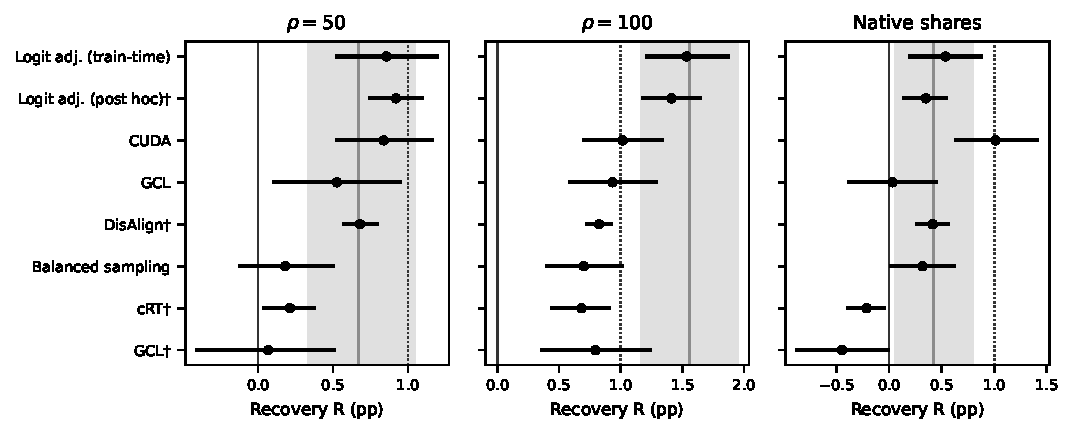
\includegraphics[width=\textwidth]{fig_recovery.pdf}
  \caption{Logit adjustment recovers the full damage at $\rho=50$ and $\rho=100$; at native shares only CUDA gains a point. Paired recovery $R_m$ with 95\% intervals. The grey line and band mark the CE damage $D$ with its interval, the solid line zero, and the dotted line the one-point threshold. $^{\dagger}$Classifier only.}
  \label{fig:recovery}
\end{figure}

\begin{table}[t]
\centering
\footnotesize
\setlength{\tabcolsep}{3.5pt}
\resizebox{\textwidth}{!}{%
\begin{tabular}{@{}lccccc@{}}
\toprule
& \multicolumn{2}{c}{$\rho=50$ ($D=0.67$)} & \multicolumn{2}{c}{$\rho=100$ ($D=1.56$)} & N ($D=0.42$) \\
\cmidrule(lr){2-3}\cmidrule(lr){4-5}\cmidrule(lr){6-6}
Method & $R_m$ & share & $R_m$ & share & $R_m$ \\
\midrule
Logit adj.\ (train-time) & 0.86 $[0.53, 1.19]$ & 1.27 $[0.81, 2.25]$ & \textbf{1.54} $[1.21, 1.87]$ & 0.99 $[0.80, 1.24]$ & 0.54 $[0.20, 0.88]$ \\
Logit adj.\ (post hoc)$^{\dagger}$ & 0.92 $[0.75, 1.10]$ & 1.37 $[0.95, 2.55]$ & \textbf{1.41} $[1.18, 1.65]$ & 0.91 $[0.75, 1.13]$ & 0.35 $[0.14, 0.54]$ \\
CUDA & 0.84 $[0.52, 1.16]$ & 1.25 $[0.74, 2.45]$ & \textbf{1.02} $[0.70, 1.34]$ & 0.65 $[0.45, 0.89]$ & \textbf{1.01} $[0.63, 1.41]$ \\
GCL & 0.41 $[0.02, 0.78]$ & 0.60 $[0.05, 1.13]$ & 0.95 $[0.54, 1.35]$ & 0.61 $[0.38, 0.84]$ & 0.23 $[-0.18, 0.65]$ \\
DisAlign$^{\dagger}$ & 0.68 $[0.58, 0.79]$ & 1.01 $[0.69, 1.90]$ & 0.83 $[0.73, 0.92]$ & 0.53 $[0.43, 0.68]$ & 0.42 $[0.27, 0.56]$ \\
Balanced sampling & 0.18 $[-0.12, 0.50]$ & 0.27 $[-0.29, 0.68]$ & 0.70 $[0.40, 1.01]$ & 0.45 $[0.28, 0.62]$ & 0.32 $[0.01, 0.62]$ \\
cRT$^{\dagger}$ & 0.21 $[0.04, 0.37]$ & 0.32 $[0.07, 0.62]$ & 0.68 $[0.45, 0.91]$ & 0.44 $[0.31, 0.59]$ & $-0.21$ $[-0.39, -0.05]$ \\
GCL$^{\dagger}$ & $-0.35$ $[-0.73, 0.02]$ & $-0.52$ $[-1.80, 0.03]$ & $-0.20$ $[-0.62, 0.23]$ & $-0.13$ $[-0.48, 0.13]$ & $-0.07$ $[-0.46, 0.34]$ \\
\bottomrule
\end{tabular}}
\caption{At $\rho=100$ the share intervals of both forms of logit adjustment include 1; every other share interval ends below it. Recovery $R_m$ in BA points and share of the CE damage, with paired 95\% intervals; bold marks material recovery ($R_m\geq1$, interval above zero). $^{\dagger}$Classifier only, frozen encoder; unmarked rows train end to end. Shares at native shares are omitted because the damage there is too small for a stable ratio.}
\label{tab:recovery}
\end{table}

\subsection{Imbalance-specific recovery}
The balanced gains point in opposite directions (Table~\ref{tab:specific}). CUDA reaches 72.32 percent BA on the balanced allocation, a gain of $G=0.81$ points $[0.48, 1.14]$ over CE. End-to-end GCL ($-0.55$ $[-0.87, -0.24]$), its classifier-only form ($-0.60$ $[-0.94, -0.27]$), and cRT ($-0.41$ $[-0.54, -0.28]$) lower balanced accuracy, all with intervals below zero; DisAlign is indistinguishable from CE.

Net of these gains, CUDA corrects none of the imbalance. Its imbalance-specific recovery is 0.20 points $[-0.17, 0.57]$ at $\rho=100$, 0.03 at $\rho=50$, and 0.20 at native shares, all with intervals that include zero. The methods with a negative balanced gain correct more than their recovery against CE shows. End-to-end GCL corrects 1.49 points $[1.00, 1.99]$ at $\rho=100$, a share of 0.96 $[0.71, 1.21]$, and cRT 1.10 points $[0.85, 1.34]$, a share of 0.71; both are material. Classifier-only GCL stays unresolved at 0.40 points $[-0.10, 0.91]$, and DisAlign's 0.83 points are unchanged. On this reading four variants are material at $\rho=100$: both forms of logit adjustment, whose $G_m$ is zero, end-to-end GCL, and cRT. CUDA drops out.

\begin{table}[t]
\centering
\small
\resizebox{\textwidth}{!}{%
\begin{tabular}{@{}lccccc@{}}
\toprule
& & \multicolumn{3}{c}{$R_m-G_m$} & $\rho=100$ \\
\cmidrule(lr){3-5}\cmidrule(lr){6-6}
Method & $G_m$ & $\rho=50$ & $\rho=100$ & N & share \\
\midrule
CUDA & 0.81 $[0.48, 1.14]$ & 0.03 $[-0.30, 0.37]$ & 0.20 $[-0.17, 0.57]$ & 0.20 $[-0.23, 0.63]$ & 0.13 $[-0.13, 0.34]$ \\
GCL & $-0.55$ $[-0.87, -0.24]$ & 0.96 $[0.51, 1.40]$ & \textbf{1.49} $[1.00, 1.99]$ & 0.78 $[0.27, 1.30]$ & 0.96 $[0.71, 1.21]$ \\
GCL$^{\dagger}$ & $-0.60$ $[-0.94, -0.27]$ & 0.25 $[-0.21, 0.71]$ & 0.40 $[-0.10, 0.91]$ & 0.53 $[0.04, 1.05]$ & 0.26 $[-0.08, 0.53]$ \\
cRT$^{\dagger}$ & $-0.41$ $[-0.54, -0.28]$ & 0.63 $[0.43, 0.82]$ & \textbf{1.10} $[0.85, 1.34]$ & 0.20 $[0.00, 0.41]$ & 0.71 $[0.56, 0.92]$ \\
DisAlign$^{\dagger}$ & $0.00$ $[-0.01, 0.01]$ & 0.68 $[0.58, 0.79]$ & 0.83 $[0.73, 0.92]$ & 0.42 $[0.27, 0.56]$ & 0.53 $[0.43, 0.68]$ \\
\bottomrule
\end{tabular}}
\caption{Net of its effect on the balanced allocation, CUDA corrects none of the imbalance, whereas end-to-end GCL and cRT correct more than their recovery against CE shows. Balanced gain $G_m$ and imbalance-specific recovery $R_m-G_m$ (Eq.~\ref{eq:specific}) in BA points, with its share of the CE damage at $\rho=100$; paired 95\% intervals, bold marks material recovery. $^{\dagger}$Classifier only. Balanced sampling and logit adjustment have $G_m=0$ by construction, so their $R_m$ in Table~\ref{tab:recovery} is already imbalance-specific.}
\label{tab:specific}
\end{table}

\subsection{End-to-end versus classifier-only training}
The two matched pairs behave differently. Post-hoc logit adjustment, applied to the CE model at inference without retraining, recovers nearly as much as its train-time form (1.41 against 1.54 points at $\rho=100$, 0.92 against 0.86 at $\rho=50$). Re-fitting GCL's classifier, in contrast, loses the recovery that end-to-end GCL achieved: 0.95 points become $-0.20$ at $\rho=100$, and 0.41 become $-0.35$ at $\rho=50$. This pair drives the family means, 0.67 for end-to-end and 0.44 for classifier-only methods at $\rho=100$. Without the two GCL variants the means are 0.70 and 0.63. These family and pair comparisons are point estimates without intervals.

\subsection{Where recovery lands}
At $\rho=100$ the CE model keeps 61.2 percent recall in the tail third of classes by assigned rank, against 71.6 percent when balanced, and gains 6.3 points in the head (Figure~\ref{fig:rank}). Only logit adjustment restores most of the tail, to 69.4 (train-time) and 69.9 percent (post hoc), paid for by about four points of head recall. End-to-end GCL and cRT raise the tail to about 66 percent, and DisAlign and balanced sampling to about 65. CUDA does not rebalance: it raises head and body by 0.7 points and the tail by 1.7, and its tail stays at 62.9 percent. Classifier-only GCL lowers the tail to 60.2 percent, below CE, and gains in the body instead. Rank-group recalls are point estimates.

\begin{figure}[t]
  \centering
  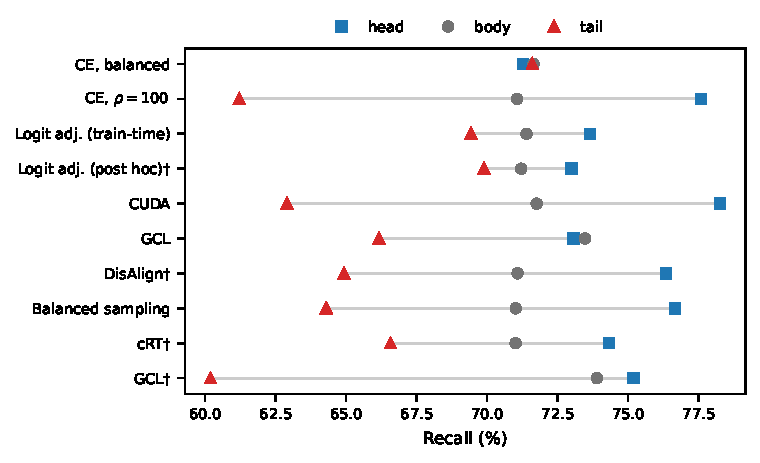
\includegraphics[width=0.72\textwidth]{fig_rank_recall.pdf}
  \caption{Only logit adjustment brings tail recall back near the balanced level at $\rho=100$; CUDA shifts all three groups upward and leaves the spread of CE. Patient-macro recall of the head, body, and tail thirds of classes by assigned rank, averaged over shards. $^{\dagger}$Classifier only.}
  \label{fig:rank}
\end{figure}

\subsection{Selected strengths}
Validation selection favours mild corrections. At $\rho=100$, logit adjustment selects half the prior correction, $\tau=0.5$, in 17 of 30 shards in its train-time form and in 20 of 30 post hoc; the full correction $\tau=1$ wins 9 and 10 shards, and $\tau=0.25$ wins 4 and none. CUDA selects its lowest augmentation probability, $p_{\mathrm{aug}}=0.25$, in 17 of 30 shards and never $p_{\mathrm{aug}}=1$; on the balanced allocation it selects 0.25 in 20 of 30. GCL selects $\sigma=0.05$ in 25 of 30 shards in both forms, DisAlign $\gamma=1.5$ in 19, and balanced sampling full balancing $s=1$ in 19. The selections at $\rho=50$ resemble those at $\rho=100$, except that DisAlign splits evenly between $\gamma=1.5$ and its largest value $\gamma=2$ (14 shards each). At native shares, DisAlign selects its largest value $\gamma=3$ in 16 of 30 shards, and train-time logit adjustment spreads over all three values (9, 8, and 13 shards).

\subsection{Probability quality}
Imbalance does not worsen the raw probabilities of the LoRA model, which are overconfident at every allocation. The balanced CE model has a raw NLL of 1.37 nats and a raw ECE of 16.8 points; at $\rho=100$ the values are 1.32 and 16.0. Temperature scaling removes most of this miscalibration and reveals a small cost of imbalance: scaled NLL rises from 1.03 to 1.07 nats and scaled ECE from 2.3 to 3.4 points. CUDA has by far the lowest raw NLL, 1.08 nats $[1.02, 1.15]$, and raw ECE, 11.5 points $[10.5, 12.6]$, at $\rho=100$; cRT (1.48) and balanced sampling (1.43) are highest. After scaling, every method lies between 0.98 (CUDA) and 1.07 nats, and scaled ECE lies between 1.7 points (post-hoc logit adjustment) and 3.5 points (classifier-only GCL). The scaled intervals are unpaired and overlap. CUDA's augmentation curbs raw overconfidence, but temperature scaling brings every other method close to it.

\section{Discussion}
\label{sec:discussion}
\textbf{How much does each method recover?} On TCGA-UT, logit adjustment closes the gap. At $\rho=100$ both of its forms recover the full 1.56 points within the uncertainty of the paired share, and they restore tail recall from 61 to almost 70 percent. No other method reaches the full damage: CUDA, end-to-end GCL, DisAlign, balanced sampling, and cRT recover between two-fifths and two-thirds of it. At $\rho=50$ and at native shares the damage is below one point, so every difference between methods there is smaller than the practical threshold of this study.

\textbf{Is CUDA's gain an imbalance correction?} No. CUDA improves the balanced model by 0.81 points, and its recoveries of 0.84, 1.02, and 1.01 points at $\rho=50$, $\rho=100$, and native shares are about the same size. Its imbalance-specific recovery is indistinguishable from zero at every allocation, and it leaves the gap between head and tail recall as wide as under CE. It is nevertheless useful: at native shares it gives the most accurate model of the study, 72.10 percent, and it has the best raw probabilities at every imbalanced allocation. CUDA is a general improvement of the LoRA model and can be combined in principle with a prior correction, which this study did not test.

\textbf{Which conclusions carry over from BRACS?} Four do. Logit adjustment is the only method that substantially restores tail recall. Its post-hoc form, a fixed prior subtraction at inference, matches its train-time form. CUDA's gain is mostly or entirely general. GCL and cRT make the balanced model slightly worse and are less damaged by imbalance than their recovery against CE suggests. Three conclusions do not carry over. On BRACS no method closed the gap, and logit adjustment recovered about two-fifths of a 4.95-point damage; on TCGA-UT it recovers all of a 1.56-point damage. CUDA gave the most accurate model at $\rho=100$ on BRACS but ranks third here, because its general gain is smaller than the imbalance-specific correction of logit adjustment. And classifier-only GCL, which gave the largest imbalance-specific correction on BRACS, recovers nothing on TCGA-UT, so the two GCL forms are not interchangeable. Validation also selects a weaker prior correction, $\tau=0.5$ instead of $\tau=1$. These comparisons are descriptive, because the datasets differ in class count, patient support, and training length.

\textbf{Why is the gap closable here?} The study does not test this, but the result fits the frozen-readout analysis of TCGA-UT \citep{queisler2026causeTcga}. There the frequency effect alone was the largest single source of damage, and thin tail support cost little by itself and mainly amplified the frequency effect. A method that removes the frequency effect then also removes most of the interaction. Under LoRA the damage is smaller to begin with, and at $\rho=100$ the tail still keeps 61 percent recall, so the model has learned the rare classes and mainly misplaces their decision boundary. On BRACS the tail fell to 5 percent recall, which a shift of the boundary cannot repair.

\textbf{Does LoRA itself help?} Partly. Under LoRA the damage at $\rho=100$ is 1.56 instead of 2.91 points. Of that difference of 1.35 points, 0.55 come from a less accurate balanced model and 0.81 from a more accurate imbalanced model, mostly in body and tail recall. The best mitigated model at $\rho=100$, train-time logit adjustment at 71.49 percent, stays 0.57 points below the frozen balanced readout. Adaptation therefore does not raise the accuracy available on balanced data, but it does make the encoder less sensitive to imbalance on TCGA-UT, which it did not on BRACS.

\textbf{Limitations.} The study covers one dataset, one encoder, and one adaptation scheme. The training length is the largest candidate tested, and validation accuracy was still rising slowly at 2,400 steps (69.1 to 69.8 percent from 1,200), so the LoRA models may not be converged; a longer training could change the balanced reference and thus every damage. Three selections concentrate on a grid edge that could be extended and was not: CUDA's lowest augmentation probability at every allocation, and DisAlign's largest $\gamma$ at native shares and, in part, at $\rho=50$. A wider grid could raise these two methods' recoveries, so their values are lower bounds on what the methods can reach. The damages at $\rho=50$ and native shares are below one point, which makes the shares there unstable and the one-point criterion uninformative. Imbalance-specific recovery assumes that a method's effect on the balanced allocation carries over additively to the imbalanced ones, which the design does not test. The comparisons with the frozen readout and with BRACS are descriptive and have no paired intervals.


\bibliographystyle{plainnat}
\bibliography{references}
\end{document}
